%#suvash#
Collaborative filtering algorithms suffer from the user cold-start problem,
where no historical information about user is available. One of the advantage of SAF is that 
the social affinity features for a user-item are defined in terms of the user's affinity groups(ASAG/ISAG).
Hence, the SAF learning is quite independent of individual user's data. 

For user cold-start analysis, we create 10 fold train-test set where users in train and test set are mutually exclusive
and each test set consists of 10\% of the total users. We hold out 30\% of each user's data from the test set 
and train two SAF predictors namely: \textit{cold-start} and \textit{non cold-start} predictor.
We train cold-start predictor using training set, whereas non cold-start predictor is trained with additional 
held out data from test set. Finally, we evaluate the performance of cold-start and non cold-start predictor on remaining 70\% 
of test data. In fig~\ref{fig:coldstart} we clearly see that the accuracy \footnote{ The slight decrease in accuracy for non cold-start case compared to 
fig~\ref{Fig1} is due to the fact that the training set consists of only 30\% of test set users data and test 
set is biased to small set of test users.} of  SAF predictor for cold-start is always better than constant predicotor and is comparable
to non cold-start case, which indicates that SAF performs quite well for cold-start users where most of the
existing methods fail.  Hence, unlike standard (social) collaborative filtering techniques, SAF is robust to user 
cold-start problem.  


\begin{figure*}[tbp!]
\centering
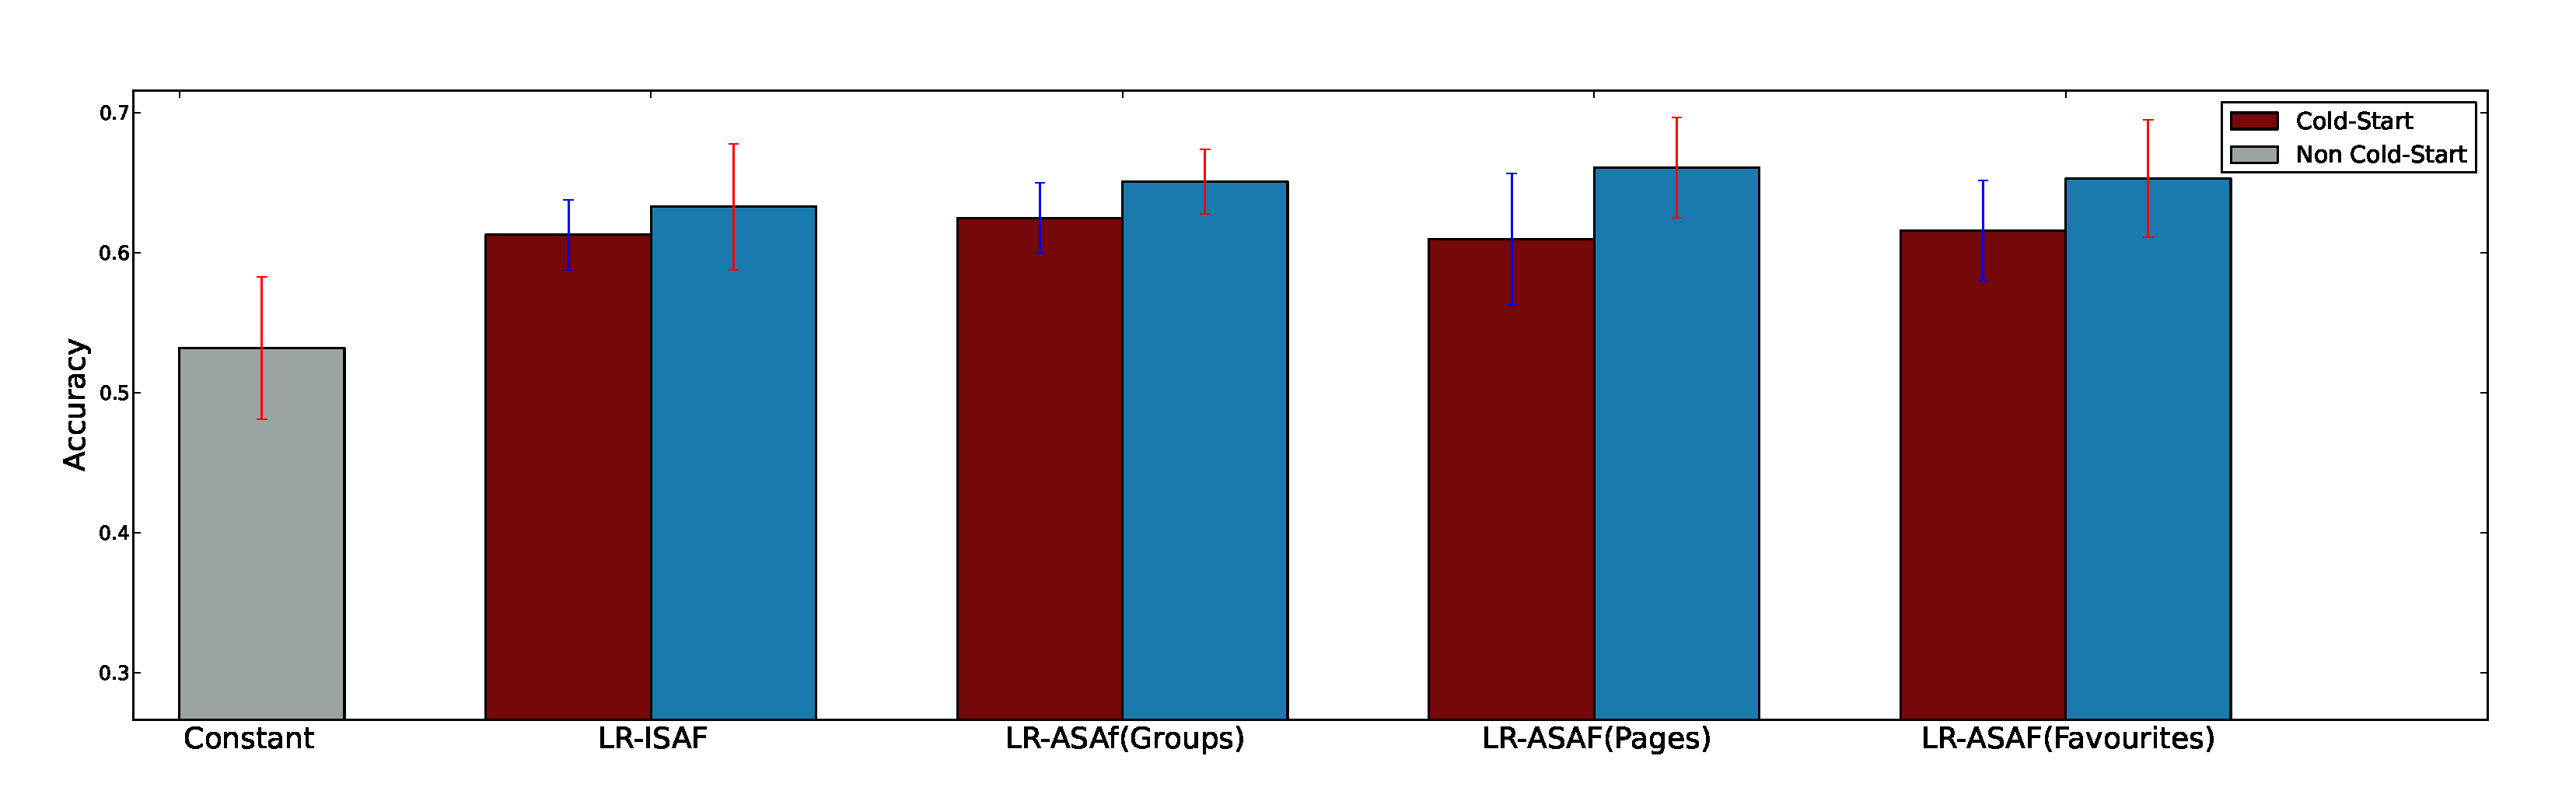
\includegraphics[width=180mm,height=50mm]{data/plots/new/cold_start.eps}
\vspace{-3mm}
\caption{Comparision of the SAF for user cold-start and non cold-start cases.
For each SAF predictor, accuracy of the predictor evaluated on user
cold start case is comparable to the accuracy of predictor for non-cold start case.}
\label{fig:coldstart}
\end{figure*}
 
%\begin{table}[t!]
%\centering
%\begin{tabular}{|>{\small}l|>{\small}r|>{\small}r|}
%\hline
%& \multicolumn{2}{|c|}{\textbf{Accuracy}}\\
%\hline
%\textbf{Predictor}& \textbf{Cold-Start} & \textbf{Non Cold-Start}\\
%\hline
%\textbf{Constant} & 0.526  +/-  0.063 & 0.526  +/-  0.063 \\
%\hline
%\textbf{LR-ISAF} & 0.613 +/- 0.025 & 0.633  +/-  0.045 \\
%\hline
%\textbf{LR-ASAF(Groups)} & 0.625  +/-  0.025 & 0.651  +/-  0.023 \\
%\hline
%\textbf{LR-ASAF(Pages)} & 0.601  +/-  0.067 & 0.655  +/-  0.036 \\
%\hline
%\textbf{LR-ASAF(Favourites)} & 0.616  +/-  0.049 & 0.653  +/-  0.042\\
%\hline
%\end{tabular}
%\caption{Comparision of performance of SAF for user cold-start and non cold-start case}
%\label{tab:coldstart}
%\end{table}